% A procedure for testing a model on an ecological task.
% ---------------------------------------------------------------------------
% style.tex --- shared preamble for every figure in book/figures/tikz/
%
% One style for all figures: Latin Modern, thin black lines, a light grey
% fill, and one accent colour used only to mark what is untrusted or wrong.
% Build with scripts/build_figures.sh; see book/figures/README.md.
% ---------------------------------------------------------------------------
\documentclass[tikz,border=6pt]{standalone}
\usepackage[T1]{fontenc}
\usepackage{lmodern}
\usetikzlibrary{arrows.meta,positioning,shapes.geometric,calc,fit,backgrounds}

\hyphenpenalty=10000   % short lines in boxes: ragged, never hyphenated

\definecolor{lightgrey}{gray}{0.92}
\definecolor{accent}{HTML}{9B2D20}

\tikzset{
  every picture/.style={
    line width=0.6pt,
    font=\small,
    >={Stealth[length=5pt,width=4pt]},
    node distance=14pt and 24pt,
  },
  % shapes
  box/.style={draw, rectangle, inner xsep=8pt, inner ysep=5pt,
              minimum height=22pt, align=center},
  grey/.style={box, fill=lightgrey},
  rounded/.style={box, rounded corners=9pt},
  decision/.style={draw, diamond, aspect=2.4, inner sep=1.5pt, align=center},
  group/.style={draw, dashed, rounded corners=5pt, inner sep=7pt},
  % text
  tag/.style={font=\footnotesize, align=center, inner sep=2pt},
  note/.style={font=\footnotesize\itshape, align=center, inner sep=2pt},
  code/.style={font=\small\ttfamily},
  codetag/.style={font=\footnotesize\ttfamily, align=center, inner sep=2pt},
  title/.style={font=\small\scshape, align=center, inner sep=2pt},
  % lines
  arrow/.style={->},
  back/.style={->, dashed},
  thin/.style={line width=0.4pt, gray},
  % the one accent, for what is untrusted, wrong or missing
  bad/.style={accent},
  badbox/.style={box, draw=accent, text=accent},
}

\begin{document}
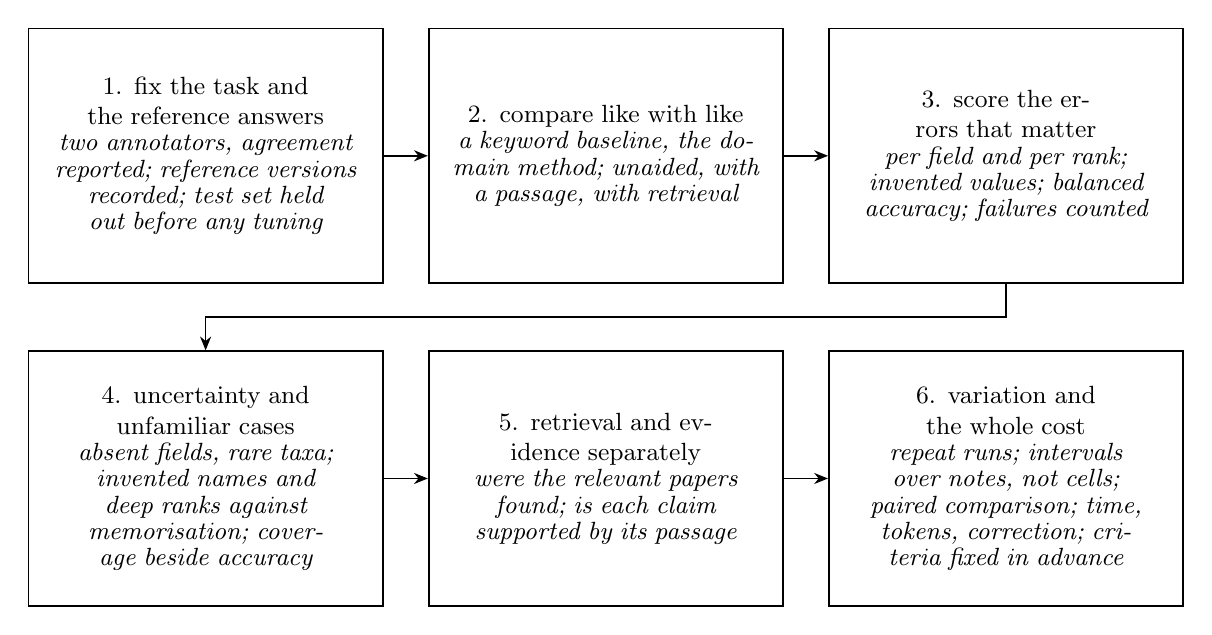
\begin{tikzpicture}[node distance=24pt and 16pt,
                    stage/.style={box, text width=112pt, align=center, font=\footnotesize,
                                  minimum height=92pt}]
  \node[stage] (s1) {\small 1. fix the task and the reference answers\\ \itshape two annotators, agreement reported; reference versions recorded; test set held out before any tuning};
  \node[stage, right=of s1] (s2) {\small 2. compare like with like\\ \itshape a keyword baseline, the domain method; unaided, with a passage, with retrieval};
  \node[stage, right=of s2] (s3) {\small 3. score the errors that matter\\ \itshape per field and per rank; invented values; balanced accuracy; failures counted};
  \node[stage, below=of s1] (s4) {\small 4. uncertainty and unfamiliar cases\\ \itshape absent fields, rare taxa; invented names and deep ranks against memorisation; coverage beside accuracy};
  \node[stage, right=of s4] (s5) {\small 5. retrieval and evidence separately\\ \itshape were the relevant papers found; is each claim supported by its passage};
  \node[stage, right=of s5] (s6) {\small 6. variation and the whole cost\\ \itshape repeat runs; intervals over notes, not cells; paired comparison; time, tokens, correction; criteria fixed in advance};
  \draw[->] (s1) -- (s2); \draw[->] (s2) -- (s3);
  \draw[->] (s3.south) -- ++(0,-12pt) -| (s4.north);
  \draw[->] (s4) -- (s5); \draw[->] (s5) -- (s6);
\end{tikzpicture}
\end{document}
